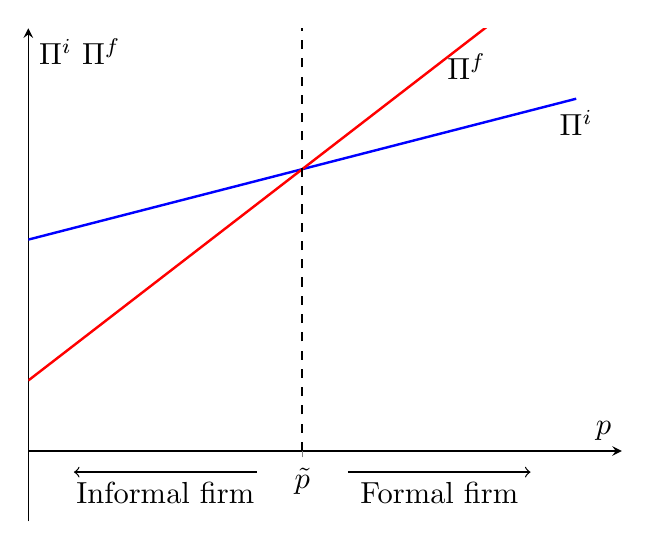
\begin{tikzpicture}[scale=1.1, transform shape]
\begin{axis}[
    axis lines=middle,
    xlabel=$p$,
    ylabel=$\Pi^i$ $\Pi^f$,
    xmin=0,
    ymin=-1,
    xmax=6.5,
    ymax=6,
    legend pos=outer north east,
    grid=none,
    xtick=\empty,  % Remove x-axis tick labels and ticks
    ytick=\empty,  % Remove y-axis tick labels and ticks
    extra x ticks={3},
    extra x tick labels={$\tilde{p}$},
]

% Plot the initial portion (y=0)
\addplot[domain=0:6, blue, thick, samples=100] {(1/3)*x+3} node[pos=1, below, black] {$\Pi^i$};

% Plot the transition
\addplot[domain=0:6, red, thick, samples=100] {x+1} node[pos=0.8, below, black] {$\Pi^f$};

% Add a vertical dashed line at x=3
\draw[dashed, black, thick] (axis cs:3,0) -- (axis cs:3,6);


\draw[->] (axis cs:3.5,-0.3) -- node[below] {Formal firm} (axis cs:5.5,-0.3);
\draw[<-] (axis cs:0.5,-0.3) -- node[below] {Informal firm} (axis cs:2.5,-0.3);


\end{axis}
\end{tikzpicture}